\documentclass[12pt,letterpaper]{article}

\usepackage{graphicx,amssymb,amsmath,bm,color,multicol}
\usepackage{../newcommand}
\sloppy
\newcommand{\ignore}[1]{}

\newenvironment{proof}{\noindent{\bf Proof:}}{\qed\bigskip}

\newtheorem{theorem}{Theorem}
\newtheorem{corollary}{Corollary}
\newtheorem{lemma}{Lemma} 
\newtheorem{claim}{Claim}
\newtheorem{fact}{Fact}
\newtheorem{definition}{Definition}
\newtheorem{assumption}{Assumption}
\newtheorem{observation}{Observation}
\newtheorem{example}{Example}
\newcommand{\qed}{\rule{7pt}{7pt}}

\newcommand{\homework}[4]{
	\thispagestyle{plain} 
	\newpage
	\setcounter{page}{1}
	\noindent
	\begin{center}
		\framebox{ \vbox{ \hbox to 6.28in
				{\bf ECON 4190: Industrial Organization \hfill #1} %change course name
				\vspace{4mm}
				\hbox to 6.28in
				{\hspace{2.5in}\large\mbox{Homework #2}}
				\vspace{4mm}
				\hbox to 6.28in
				{{\it Collaborators: #3\hfill}}
			}}
		\end{center}
	}

\oddsidemargin 0in
\evensidemargin 0in
\textwidth 6.5in
\topmargin -0.5in
\textheight 9.0in

\begin{document}

% Modify this command to be your name and computing ID
\homework{Fall 2021}{$2$}{Alex Shen (as5gd), Sean Velhagen (spv5hq), Max Bresticker (mtb9sex)}

Pledge: On my honor, I pledge that I have neither given nor received help on this assignment 
Signature: \textit{Alex Shen, Sean Velhagen, Max Bresticker}

\begin{enumerate}
	
\item[a.] 

A profit-maximizing firm will seek to max $\pi(Q) = PQ - C(Q)Q$, which we can reduce to $\pi(Q) = PQ$ because Firm 1 has no costs. Since Firm 1 has control over its price $P$, we first attempt to calculate $Q(P)$, or the quantity of consumers that will buy at a given price. To do this we can graph the consumer's utility against location, which yields this:

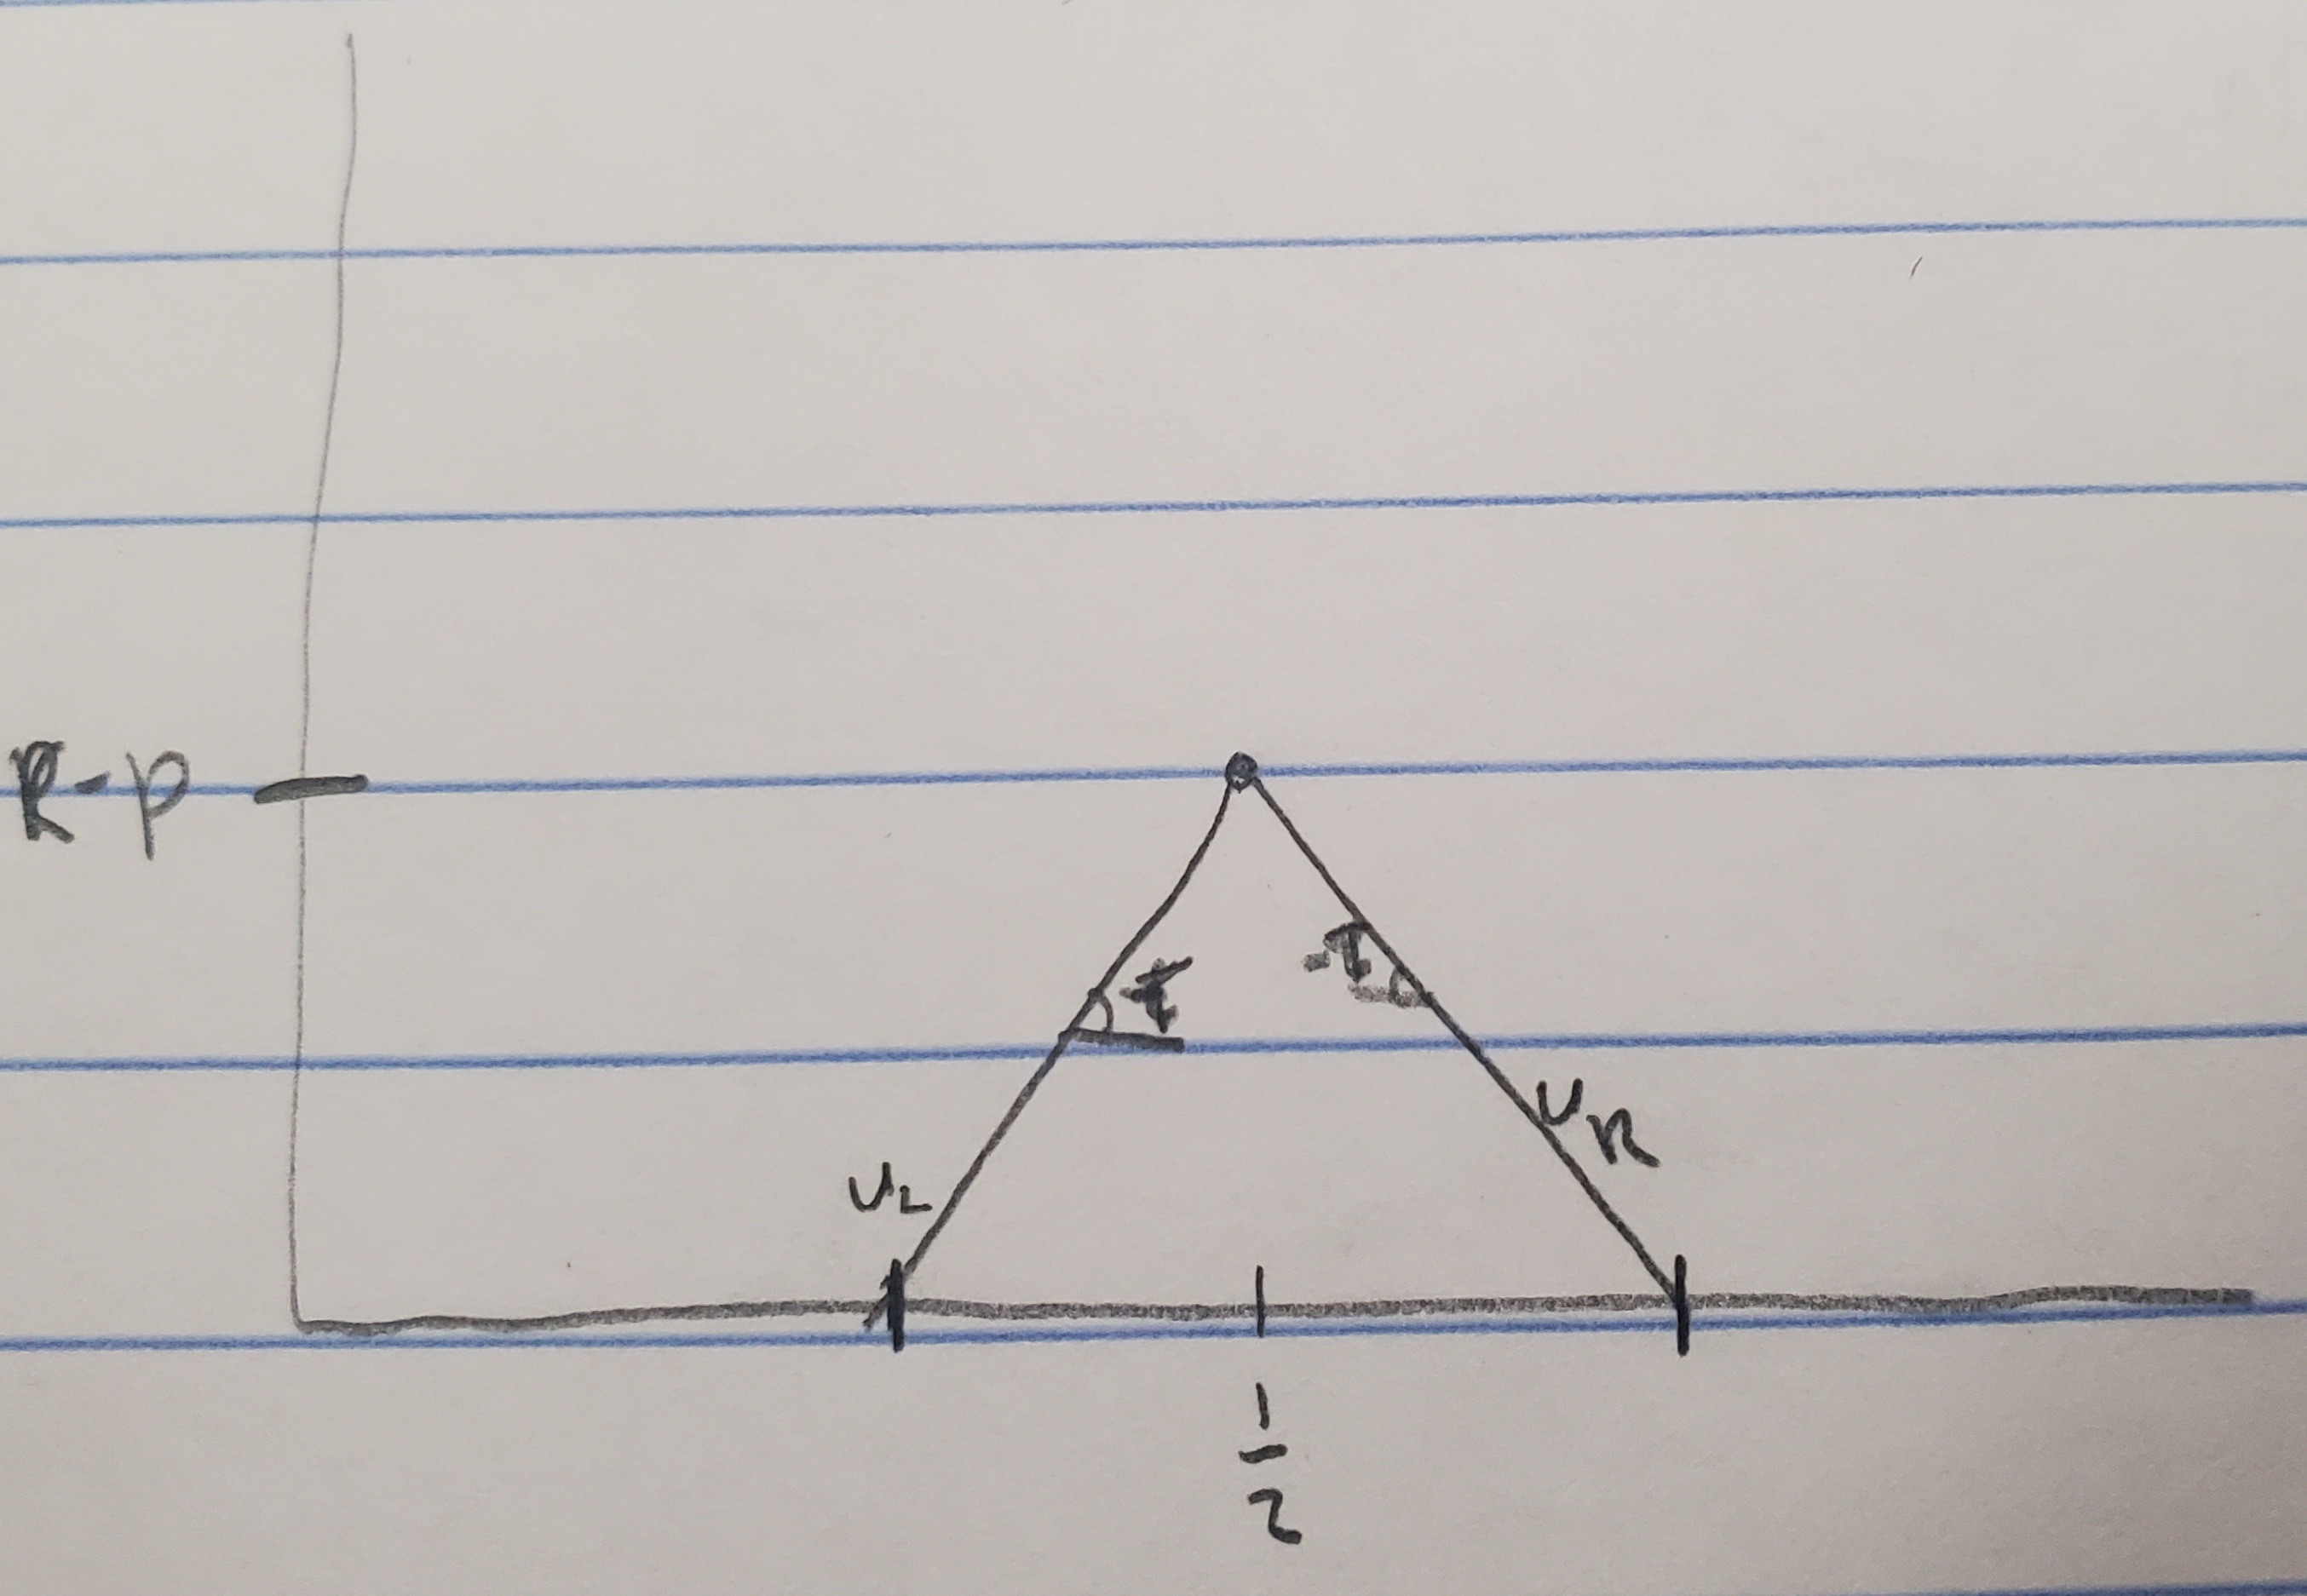
\includegraphics[scale=0.1]{a-graph.jpg}

We represent the utility of all consumers to the "left" of Firm 1 (i.e. $x<\frac{1}{2}$) with $v_l$ and all consumers to the "right" as $v_r$. They can be represented by the following equations:

\begin{align*}
v_l &= R_1 - p + T(x-\frac{1}{2}) \\
v_r &= R_1 - p - T(x-\frac{1}{2})
\end{align*}

To find $Q$, we would multiply the fraction of the market that is covered by the total mass $M$, but since $M=1$ in this case, we simply have to find the distance between the x-intercepts of $v_r$ and $v_l$: $x_r$ and $x_l$.

First solve for $x_r$ and $x_l$:
\begin{align*}
	v_l = 0 = R_1 - p + T(x-\frac{1}{2}) &\Leftrightarrow x_l = \frac{p-R_1}{T} + \frac{1}{2} \\
	v_r = R_1 - p - T(x - \frac{1}{2}) &\Leftrightarrow x_r = \frac{R_1 - p}{T} + \frac{1}{2} \\
\end{align*}

Then find the difference:

\begin{align*}
	Q(p) = x_r - x_l &= \frac{R_1 - p}{T} + \frac{1}{2} - (\frac{p-R_1}{T} + \frac{1}{2}) \\
	&= \frac{R_1 - p}{T} - \frac{p-R_1}{T} \\
	&= \frac{2R_1 - 2p}{T} \\
	Q(p) &= \frac{2}{T} (R_1 - p)
\end{align*}

Now we return to the profit function and maximize it to find the maximum price:

\begin{align*}
	max_p \pi &= p * \frac{2}{T}(R_1 - p) = \frac{2R_1p}{T} - \frac{2p^2}{T}\\
	\frac{\partial\pi}{\partial p} &= \frac{2R_1}{T} - \frac{4p}{T} = 0 \\
	&\therefore p^* = \frac{R_1}{2}
\end{align*}

Knowing price makes it easy to calculate maximum profit:
\begin{align*}
	\pi^* &= PQ = P * \frac{2}{T} (R_1 - P) \\
	&= \frac{R_1}{2} \frac{2}{T}(R_1-\frac{R_1}{2}) \\
	&= \frac{R_1}{T} * \frac{R_1}{2} \\
	&\therefore \pi^* = \frac{R_1^2}{2T}
\end{align*}

We also need to address the edge case where the market is completely covered; in that case, instead of using our previous derivations, we can use a much simpler form: since we know that the consumers at 0 and 1 are indifferent, we can use $v_l(0) = 0$ to solve for $p^*$ in this case (which also gives us profit, because $Q$ would be exactly 1):

\begin{align*}
	v_l(0) &= R_1 - p + T(-\frac{1}{2}) = 0\\
	p^* &= R_1 - \frac{T}{2} \\
	\pi^* &= R_1 - \frac{T}{2}
\end{align*}

Then Firm 1 would simply pick whichever scenario (uncovered vs. covered market) has a higher profit based on the parameters.

{\color{blue}\textbf{Solution: $p^* = \frac{R_1}{2}$, $\pi^* = \frac{R_1^2}{2T}$ when $\frac{R_1^2}{2T} > R_1 - \frac{T}{2}$, otherwise $p^*=\pi^* = R_1 - \frac{T}{2}$ }}

\item [b.] 
\end{enumerate}
	
\end{document}